\chapter{Conclusions and Future Perspectives}  \label{ch:conclusion}
\graphicspath{{conclusions/figures/}}

In this chapter, we summarize the major achievements of this thesis and we give an outlook on future perspectives.

\section{Achievements}

This thesis thouroughly describes the different steps aiming at realizing the vision of enabling self service data provisioning in the enterprise. The work presented is beneficial to both our personae introduced in the scenario (check section~\ref{section:scenario}). The contributions made are:\\

\textbf{Contributions for Data Portals Administrators}
\vspace{1mm}

Our data portal administrator \textbf{Mark} is always looking to expand his portals in terms of the number of datasets hosted, without compromising in their portal's data quality. Our proposed Harmonized Dataset Model (HDL) can act a basis to extend and present the datasets he controls. \textbf{Mark} will be able to know what are the major dataset models out there, and what kind of metadata data owners need to fully represent their dataset.

We have developed Roomba, an automatic dataset profiles generation and validation tool that can be easily extended to perform various profiling tasks. Out of the box, \textbf{Mark} can use Roomba to automatically fix datasets metadata issues, and notify the datasets owners of the other issues to be manually fixed. \textbf{Mark} will be able to identify Spam datasets resulting in higher data quality. Coming back to our scenario, the data available in the portal will no have rich semantic information attached to it. For example, temporal and spatial information extracted will be assigned into the corresponding metadata fields in HDL. As a result, various datasets will be easily identifiable to cover various parts of the UK. Moreover, the topical profilers in Roomba will be able to identify occurrences of alcohol related terms like "wine" in various datasets. Query expansion methods can be used to relate alcohol to wine.\\

\textbf{Contributions for Data Analysts}
\vspace{1mm}\\

Our data analyst \textbf{Bob} believes that "more data beats better algorithms"and is always hunting for high quality data to produce accurate reports to the management team. \textbf{Bob} will be able to have direct access to rich and high-quality dataset descriptions generated by Roomba. By examining the datasets metadata presented in HDL he will be able to make fast decisions whether the dataset examined is suitable or not. He will also have vital information about the licensing and limitations for using this data internally. He will also have assurances on the dataset quality, which will help choose the best candidates out of ranked list.
\begin{wrapfigure}{r}{0.5\textwidth}
  \begin{center}
    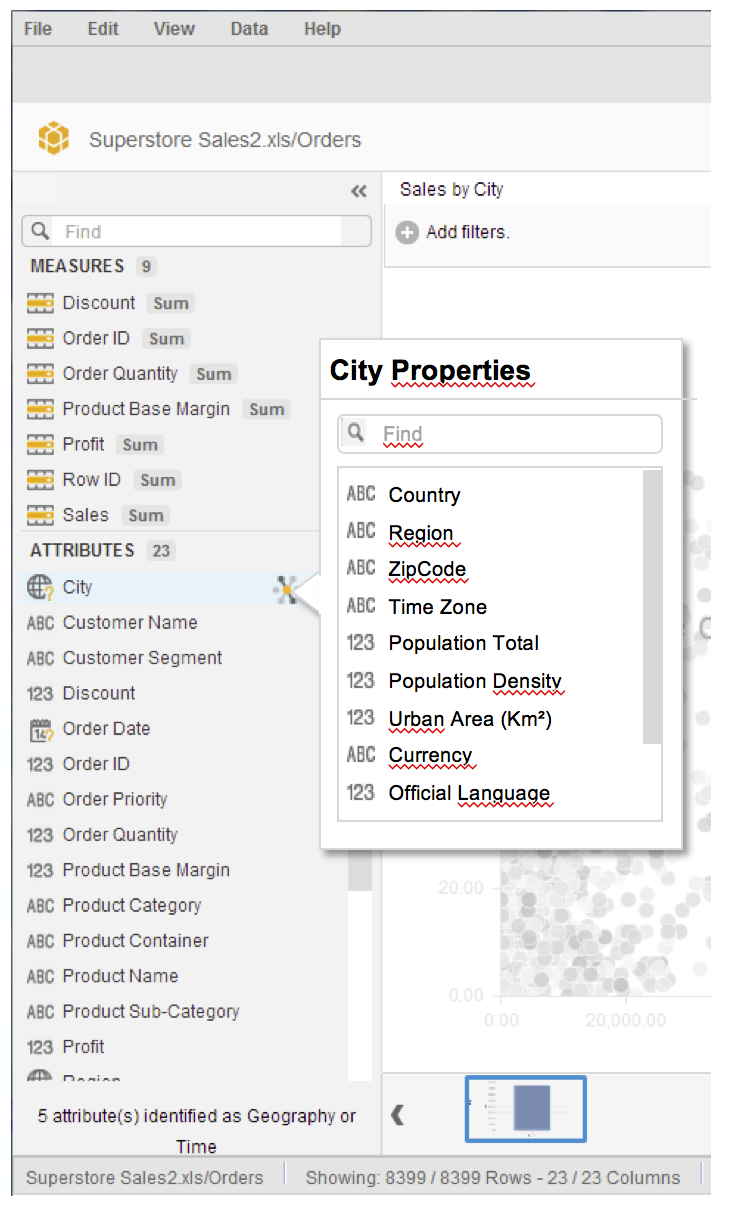
\includegraphics[width=0.48\textwidth]{lumira_sample.png}
  \end{center}
  \caption{UI Prototype of semantic data enrichment in SAP Lumira}
  \label{fig:lumira}
\end{wrapfigure}
\textbf{Bob} now has access to various datasets he found matching his query to the portal admnistered by \textbf{Mark}. Having imported those dataset into Lumira, he will be also able to use the internal knowledge base to apply various semantic enrichments on this data. Figure~\ref{fig:lumira} shows a possible integration of such service in SAP Lumira. Moreover, \textbf{Bob} will be also able to use the schema matching services to find and merge relevant datasets and reports. He can easily filter datasets by their spatial coverage. \textbf{Bob} is also a modern person, who is always trying to fresh information and believes in the wisdom of the crowd. Having SNARC services integrated with Lumira, he is also able to see a feed of relevant social media items that can be of interest to him. He actually follows a link in some tweet he saw and was able to find relevant pieces of pointers that he would like to investigate further.


In summary, the contributions above pave the way to build a set of smart services to enable analysts easily find relevant pieces of information and administrators fight Spam and be able to maintain high quality data portals. The work presented in this thesis goes beyond the fact that attaching metadata to datasets is vital, but propose a set of services that can automatically achieve that in seamless manner.

\section{Perspectives}

This thesis could be extended in th following directions:

\begin{itemize}

\item \textbf{Data Profile Representation}
\vspace{1mm}
\\
The proposed Harmonized Dataset Model (HDL) is currently available as a hierarchical JSON file. An enhancement would be to refine HDL and present it as a fully fledged OWL ontology. In addition, HDL currently contains some values that were frequently defined in CKAN extras fields. Broadening our analysis of these values by running Roomba on additional portals and present the top results as enumerations, ensuring a fine-grained representation of a dataset is a valid improvement. while we presented the mappings between various models in a table structure, an enhancement to it would be to create mappings between HDL and all the various models to ensure full compatibility. These mappings, for example, can be used to extend Roomba allowing it to perform metadata profiling on other portals like DKAN.

\item \textbf{Automatic Dataset Profiling}
\vspace{1mm}
\\
It has been noticed that the issues surrounding metadata quality affect directly dataset search as data portals rely on such information to power their search index. There are various extensions to our tool Roomba that can help in automatically building and enhancing dataset profiles. For example, integrating statistical and topical profilers to be able to generate full comprehensive profiles. Extending Roomba to be able to run over other data portal types like DKAN or Socrata by leveraging the HDL mappings. Finally, introduce workflows that will be able to correct the rest of the metadata either automatically or through intuitive manually-driven interfaces.

\item \textbf{Objective Linked Data Quality}
\vspace{1mm}
\\
Ensuring data quality in Linked Open Data is a complex process as it consists of structured information supported by models, ontologies and vocabularies and contains queryable endpoints and links. In this thesis, we managed to narrow down the set of quality issues surrounding Linked Data to those who can be objectively measured and assessed by automatic tools. Our proposed tool covers 85\% of the quality indicators proposed. A possible extension would be to integrate tools assessing models quality in addition to syntactic checkers with Roomba. This will provide a complete coverage of the proposed quality indicators. Moreover, there are currently no weights assigned to the quality indicators. A valid contribution would be to suggest weights to those indicators which will result in a more objective quality calculation process.

\item \textbf{Enterprise Data Integration}
\vspace{1mm}
\\
A vital component to Data Integration in the enterprise is the existence of enterprise knowledge bases. Integrating additional linked open data sources of semantic types such as YAGO and evaluate our matching results against instance-based ontology alignment benchmarks such as OAEI\footnote{http://oaei.ontologymatching.org/2011/instance/index.html} or ISLab\footnote{http://islab.dico.unimi.it/iimb/} are possible future directions. Moreover, our work can be generalized to data classification. The same way the AMC helps identifying the best matches for two datasets, we plan to use it for identifying the best statistical classifiers for a sole dataset, based on normalized scores.
\end{itemize}